In diesem Kapitel werden die Grundlagen in der Verwendung des Plugins erläutert. Eine Sektion führt dabei durch die Installation des Plugins und eine erläutert das Anlegen einer Frage.

\section{Installation und Aktivierung}
\label{sec:installation-und-aktivierung}

Basierend auf unterschiedlichen Ausgangssituationen und Bedürfnissen, bietet \eigenname{assSQLQuestion} zwei verschiedene Varianten der Installation. Das Plugin kann auf der einen Seite gemeinsam mit einer frischen \eigenname{ILIAS} Instanz in Form eines \eigenname{Docker}-Containers zum Laufen gebracht und auf der anderen Seite zu einer bestehenden \eigenname{ILIAS} Instanz hinzugefügt werden. Während der Ansatz mit \eigenname{Docker} vor allem zu Demonstrations- und Testzwecken gedacht ist, bietet der traditionelle Ansatz die Möglichkeit \eigenname{assSQLQuestion} in eine bestehende \eigenname{ILIAS} Instanz zu integrieren.

\subsection{Installation mit Docker}
\label{subsec:installation-mit-docker}

    \subsubsection{1. Schritt}
    
        Sollte der \eigenname{Docker} Client noch nicht auf dem gewünschten Host installiert sein, so muss dies nachgeholt werden. Eine genaue Installationsanleitung findet sich unter \url{https://docs.docker.com/install/}.
    
    \subsubsection{2. Schritt (optional)}
    
        In einem zweiten (optionalen) Schritt sollte die aktuellste Version des angebotenen \eigenname{Docker}-Images zu \eigenname{assSQLQuestion} aus der Container-Registry heruntergeladen werden. Optional ist dieser Schritt, da \eigenname{Docker} fehlende Images mit dem Starten eines Containers automatisch herunterlädt. Es sei an dieser Stelle dennoch empfohlen den Schritt nicht zu überspringen, da Docker nur so überprüft, ob eventuell eine neue Version des Images vorliegt.
        
        In diesem Fall liegt die aktuellste Version des Images unter \url{docker.gitlab.tab-e.de/qpisql/asssqlquestion:master}. Erfolgen kann das Herunterladen des Containers über:
        
        \begin{lstlisting}[language=bash]
        docker pull docker.gitlab.tab-e.de/qpisql/asssqlquestion:master
        \end{lstlisting}
    
    \subsubsection{3. Schritt}
    
        Um den \eigenname{Docker}-Container zu starten, müssen zunächst einige Variablen geklärt werden. Diese können frei vergeben werden, sollten aber auf die Umgebung angepasst sein:
        
        \begin{description}
        \item[PORT]
        Der Port auf dem die neue \eigenname{ILIAS} Instanz erreichbar sein soll. Dieser Port darf noch nicht anderweitig belegt sein.
        \item[URL] 
        Die URL oder IP auf der \eigenname{ILIAS} verfügbar gemacht wird. Wenn [PORT] zum Beispiel auf 8000 gesetzt wurde und die IP des Host-Servers 100.0.0.1 wäre, könnte hier beispielsweise 100.0.0.1:8000 als [URL] gewählt werden.
        \item[NAME]
        Der interne Name bzw. die ID des \eigenname{Docker}-Containers. 
        \end{description}
        
        Gestartet werden kann der Container mit dem Befehl:
        
        \begin{lstlisting}[language=bash]
        docker run -d \
        -p [PORT]:80 \
        -e httppath="[URL]" \
        --restart always \
        --name [NAME] \
        docker.gitlab.tab-e.de/qpisql/asssqlquestion:master
        \end{lstlisting}
    
    \subsubsection{4. Schritt}
    
        Der Container benötigt etwas Zeit um vollständig zu starten. Dies kann je nach Umgebung auch mehrere Minuten in Anspruch nehmen.
    
    \subsubsection{5. Schritt}
    
        Jetzt kann die \eigenname{ILIAS} Installation unter \textbf{[URL]} aus Schritt 2 aufgerufen werden.
    
    \subsubsection{6. Schritt}
    
        Ein Einloggen in \eigenname{ILIAS} kann unter Benutzung des Benutzernamens \glqq\textit{root}\grqq\ und des Passwortes \glqq\textit{homer123}\grqq\ erfolgen.
    
    \subsubsection{7. - 9. Schritt}

        Anschließend muss \eigenname{assSQLQuestion} aktiviert werden. Eine kurze Anleitung dazu ist in \textbf{Kapitel \ref{subsec:installation-bestehende-instanz}} zu finden.


\subsection{Installation bei einer bestehenden ILIAS Instanz}
\label{subsec:installation-bestehende-instanz}

    \subsubsection{1. Schritt}
    
        Zunächst muss der aktuelle Stand des Projektes, in unter \eigenname{Customizing/global/plugins/Modules/TestQuestionPool/Questions/assSQLQuestion} in der existierenden \eigenname{ILIAS}-Installation abgelegt werden.
    
    \subsubsection{2. - 4. Schritt}
        
        Nun muss \eigenname{assSQLQuestion} aktiviert werden. Eine kurze Anleitung dazu ist in \textbf{Kapitel \ref{subsec:installation-bestehende-instanz}} zu finden.


\subsection{Aktivierung des Plugins}
\label{subsec:aktivierung-des-plugins}

    \subsubsection{1. Schritt}
    
        Um das Plugin zu aktiveren muss unter dem Menüpunkt \glqq\textit{Administration}\grqq\ der Unterpunkt \glqq\textit{Plugins}\grqq\ aufgerufen werden.
        
            \begin{figure}[H]
                \begin{center}
                    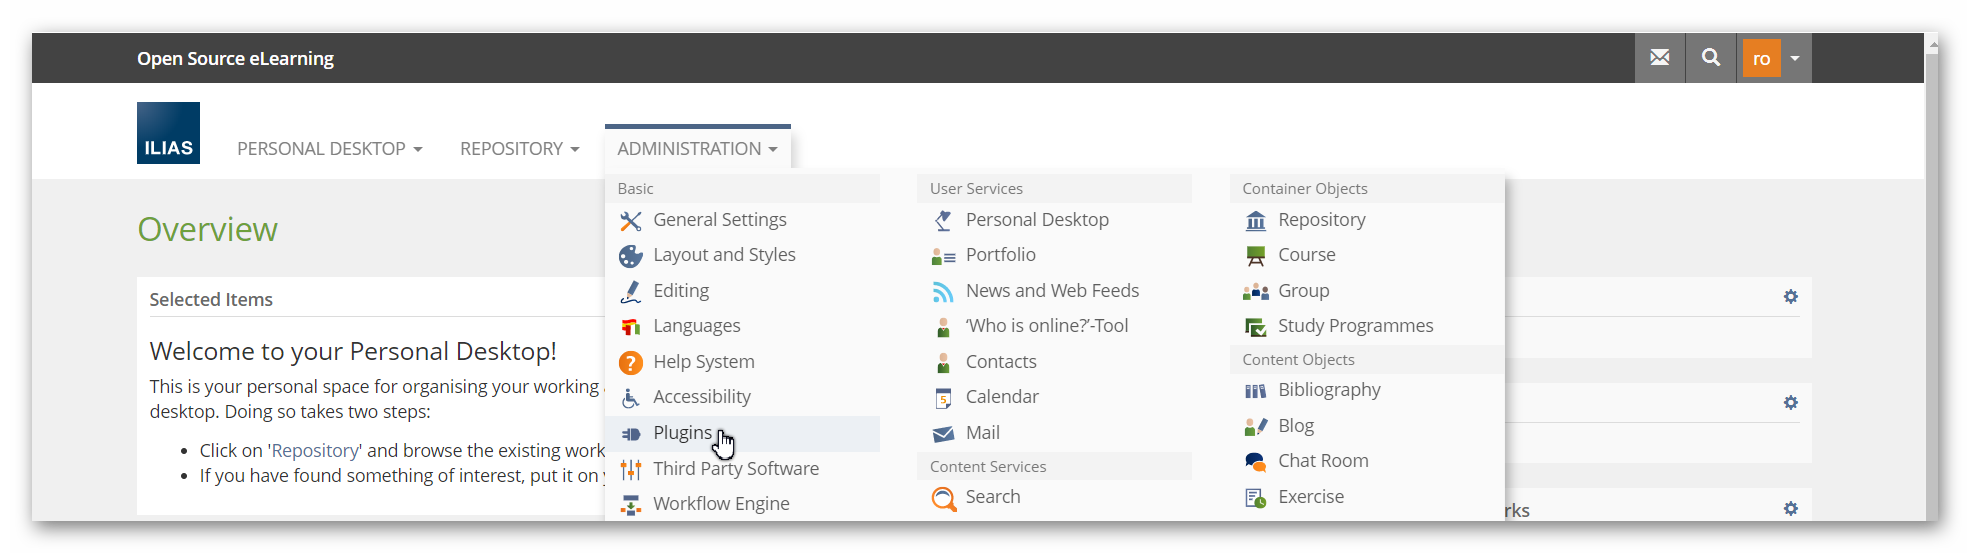
\includegraphics[page=1, width=0.7\paperwidth, trim=4 4 4 4, clip]{fig/Schritt-1-Aktivierung.png} 
                    \caption{Schritt 1 der Aktivierung des \eigenname{assSQLQuestion} Plugins}
                    \label{fig:schritt-1-aktivierung}
                \end{center}
            \end{figure}
    
    \subsubsection{2. Schritt}
    
        Die Installation von \eigenname{assSQLQuestion} erfolgt über die angezeigte \glqq\textit{Install}\grqq\ Auswahlmöglichkeit.
        
            \begin{figure}[H]
                \begin{center}
                    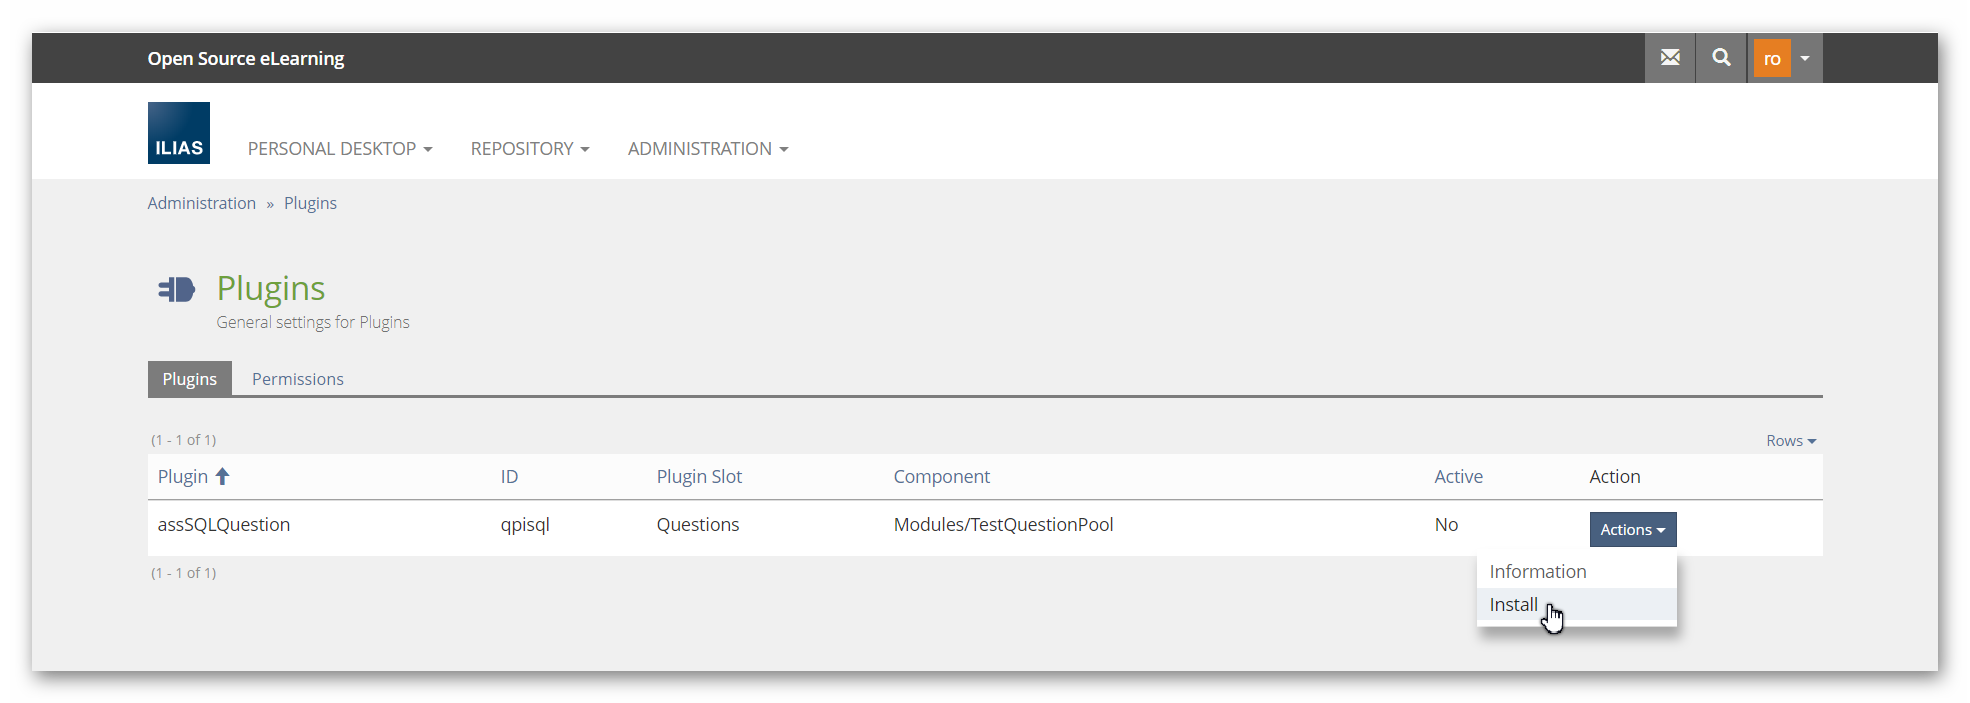
\includegraphics[page=1, width=0.7\paperwidth, trim=4 4 4 4, clip]{fig/Schritt-2-Aktivierung.png} 
                    \caption{Schritt 2 der Aktivierung des \eigenname{assSQLQuestion} Plugins}
                    \label{fig:schritt-2-aktivierung}
                \end{center}
            \end{figure}
    
    \subsubsection{3. Schritt}
    
        Abgeschlossen werden kann die Einrichtung über einen Klick auf die \glqq\textit{Activate}\grqq\ Auswahlmöglichkeit.
        
            \begin{figure}[H]
                \begin{center}
                    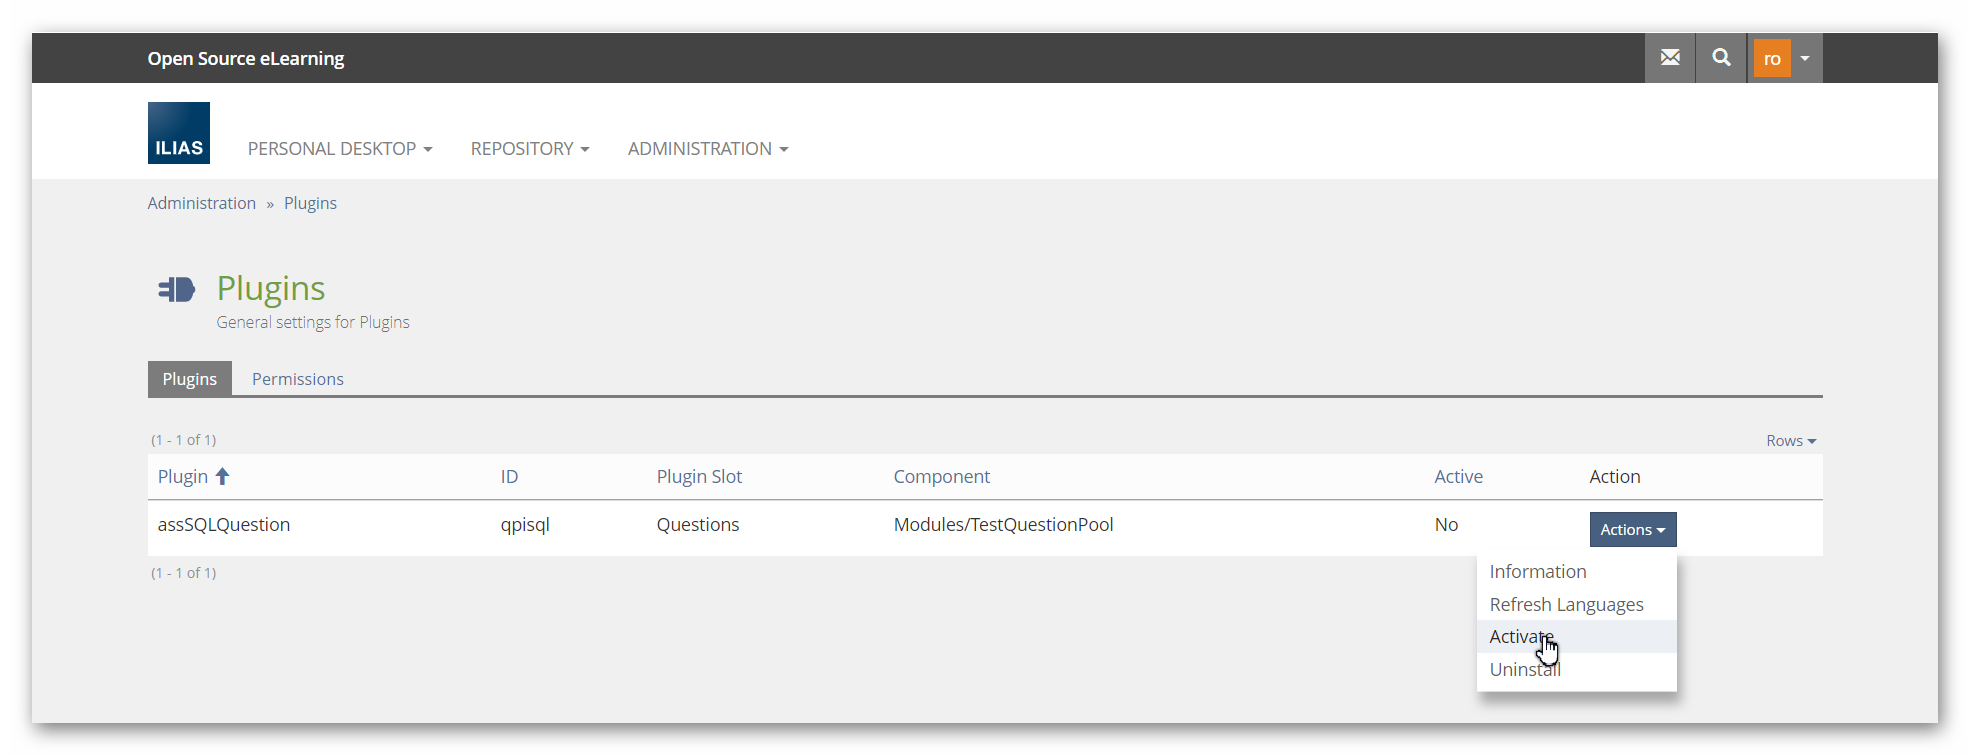
\includegraphics[page=1, width=0.7\paperwidth, trim=4 4 4 4, clip]{fig/Schritt-3-Aktivierung.png} 
                    \caption{Schritt 3 der Aktivierung des \eigenname{assSQLQuestion} Plugins}
                    \label{fig:schritt-3-aktivierung}
                \end{center}
            \end{figure}


\section{Anlegen einer Frage}
\label{sec:anlegen-einer-frage}

Das Anlegen einer allgemeinen Frage in \eigenname{ILIAS} wird grundsätzlich in der User-Dokumentation von \eigenname{ILIAS} (s. \cite{IliasAutorenDokumentation}, Kapitel 14) beschrieben. Bei der \eigenname{assSQLQuestion} gibt es aber einige Besonderheiten, die zu beachten sind. Hier wird abschnittsweise durch diese geführt.

Dabei sei zu erwähnen, dass der Fragetyp, den \eigenname{assSQLQuestion} bereitstellt, bei deutscher Spracheinstellung den Namen \glqq\textit{Interaktive SQL Frage}\grqq\ trägt. Das englische Äquivalent dazu ist in \textbf{Abbildung \ref{fig:create-question}} zu sehen und heißt \glqq\textit{Interactive SQL Question}\grqq .

    \begin{figure}[H]
        \begin{center}
            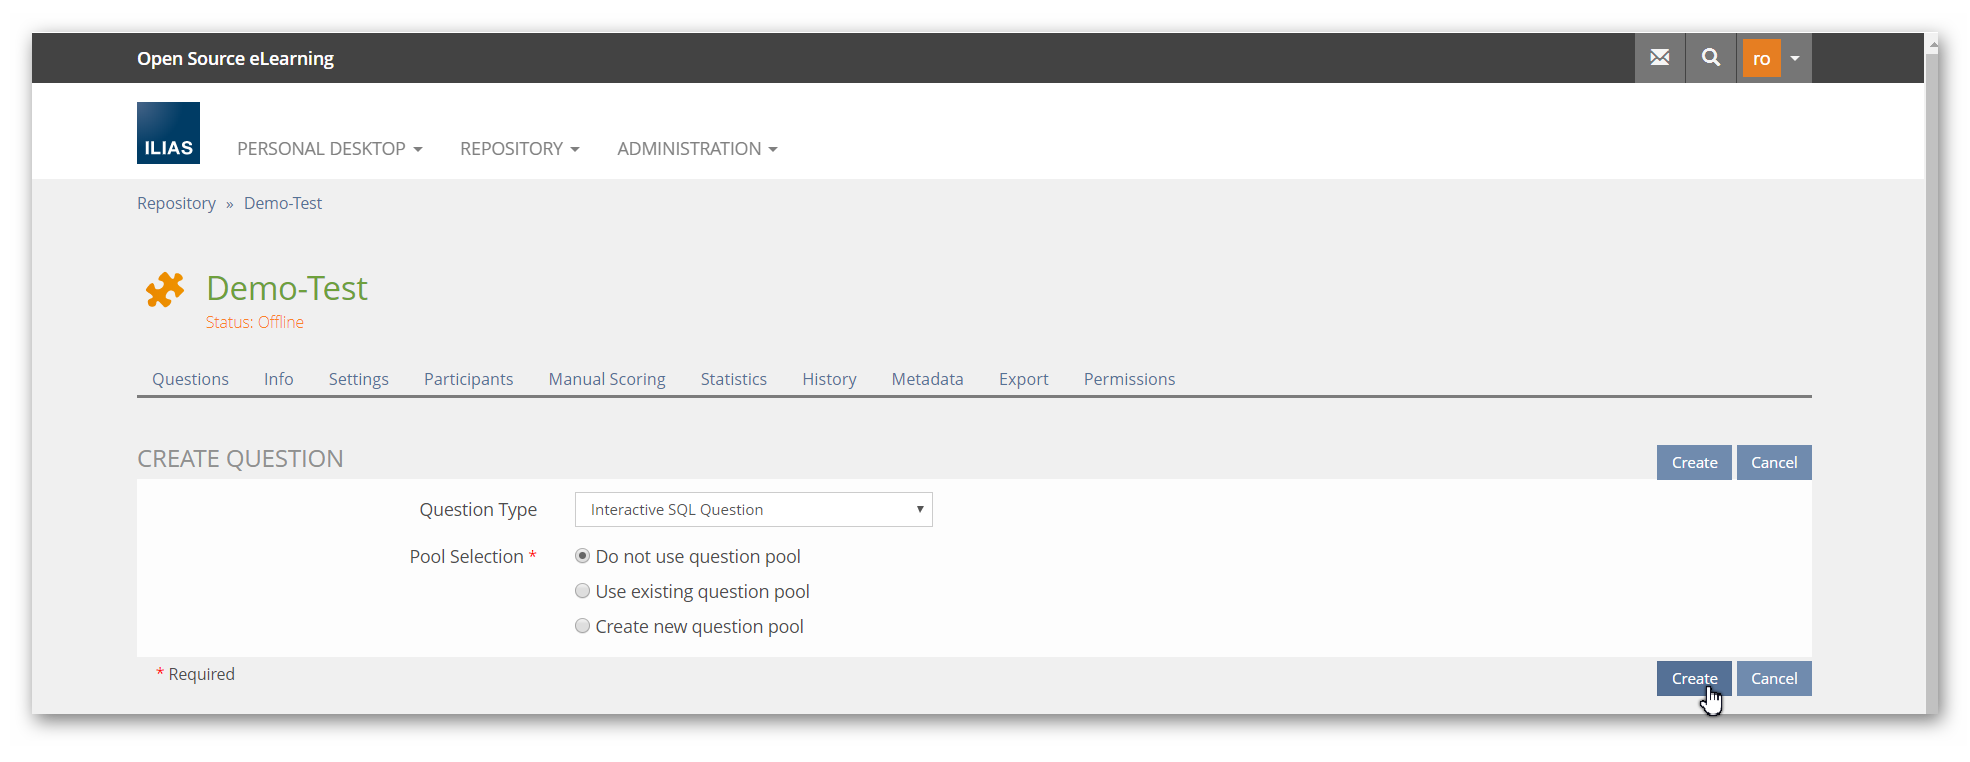
\includegraphics[page=1, width=0.7\paperwidth, trim=4 4 4 4, clip]{fig/Create-Question.png} 
            \caption{Anlegen einer neuen interaktiven SQL Frage}
            \label{fig:create-question}
        \end{center}
    \end{figure}
    
\subsection{Teil 1: Die SQL-Sequenzen}

    Der erste \eigenname{assSQLQuestion} spezifische Teil beim Anlegen einer \glqq\textit{Interaktive SQL Frage}\grqq\ sind die \glqq\textit{SQL-Sequenzen}\grqq . Dabei besteht eine \glqq\textit{Interaktive SQL Frage}\grqq\ aus bis zu drei verschiedenen dieser Sequenzen - genauer Sequenz A, B und C. Bei einer späteren Ausführung werden diese drei Sequenzen gemäß Ihrer alphabetischen Reihenfolge ausgeführt. Die Sequenzen A und C werden vom Fragenersteller vorgegeben und sind für den Teilnehmer nicht zu sehen. Sequenz B soll vom Teilnehmer später selbst erarbeitet werden. Der Fragenersteller muss dazu eine Musterlösung für diese Sequenz bereitstellen, auf deren Basis später der Teilnehmer bewertet wird. Es ist hier ebenfalls zu erwähnen, dass die automatische Korrektur von \eigenname{assSQLQuestion} nicht die Anfragen an sich bewertet, sondern die letzte sichtbare Ausgabe der SQL-Sequenzen vergleicht.
    
    Des weiteren gehört auch der sogenannte \glqq\textit{Integritätscheck}\grqq\ zum Block der \glqq\textit{SQL-Sequenzen}\grqq . Ist dieser aktiviert, werden Veränderungen an der Datenbank in Sequenz B verhindert, indem die Schlüsselworte \glqq CREATE TABLE\grqq\ , \glqq ALTER TABLE\grqq\ , \glqq DROP TABLE\grqq\ , \glqq INSERT INTO\grqq\ , \glqq UPDATE\grqq\  or \glqq DELETE FROM\grqq\ eine erfolgreiche Ausführung verhindern.
    
    Diese freie Definition wurde bewusst gewählt, um \glqq\textit{Interaktive SQL Frage}\grqq\ von zweierlei Art zu ermöglichen:
    
    \subsubsection{Frage zu einer SELECT-Anfrage}
    
        In diesem Fall nutzt der Fragenersteller Sequenz A um die Datenbank mit Inhalten zu füllen und für eine SQL Anfrage vorzubereiten. Sequenz B ist der Teil der vom Testteilnehmer beantwortet werden muss, der Ersteller füllt dennoch eine beispielhafte Sequenz ein, die als Musterlösung zu werten ist. Sequenz C wird nicht benötigt und bleibt dementsprechend leer. Da bei einer SELECT-Anfrage keine Veränderungen erwünscht sind, sollte auch der Integritätscheck aktiviert werden.
        
        \begin{figure}[H]
            \begin{center}
                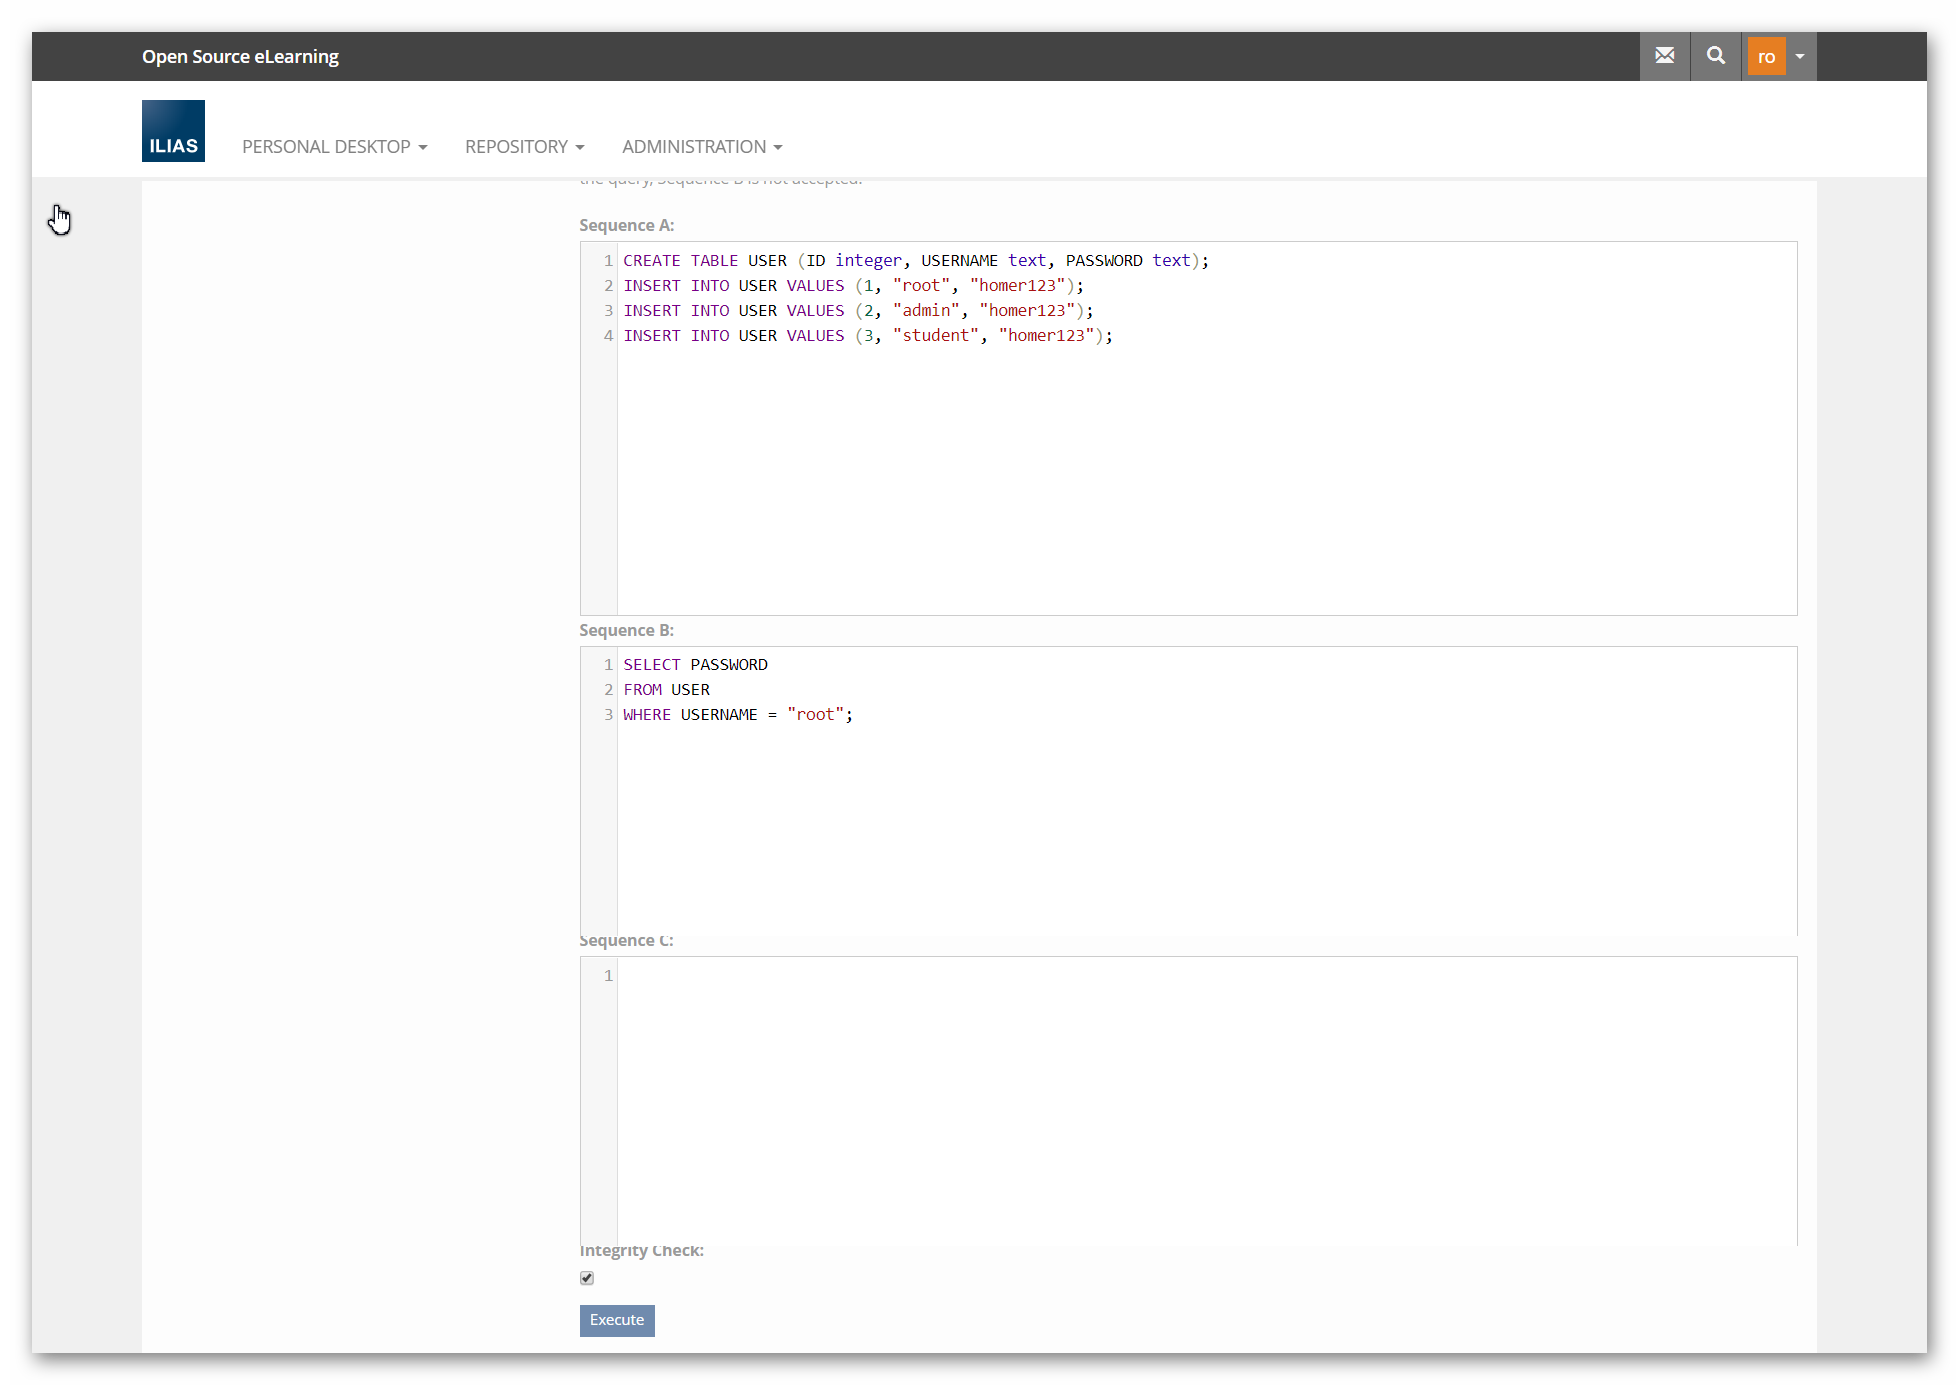
\includegraphics[page=1, width=0.7\paperwidth, trim=4 4 4 4, clip]{fig/Beispiel-SQL-Sequenzen-bei-SELECT-Anfrage.png} 
                \caption{SQL-Sequenzen im Falle einer SELECT Anfrage (Beispiel)}
                \label{fig:beispiel-sql-sequenzen-bei-select-anfrage}
            \end{center}
        \end{figure}
        
    \subsubsection{Frage zu CREATE TABLE, INSERT INTO, DELETE FROM, UPDATE, usw.}
    
        Auch in diesem Fall kann der Frageersteller Sequenz A nutzen um die Datenbank mit Inhalten zu füllen. Dies ist aber von der gewünschten Fragestellung abhängig. Sequenz B ist wieder die Sequenz, die Teilnehmer im Test selbst schreiben müssen. Da die Frage die Fähigkeiten des Teilnehmers prüfen soll CREATE TABLE, INSERT INTO, DELETE FROM, UPDATE und ähnliche Anfragen zu beantworten, wird Sequenz B in den meisten Fällen keine SELECT-Anfrage enthalten. Hier ist es wichtig, dass der Testersteller dann in Sequenz C eine Ausgabe erzeugt, da sonst keine Bewertung der Antwort möglich ist. Der Integritätscheck darf dabei nicht aktiviert sein.
        
        \begin{figure}[H]
            \begin{center}
                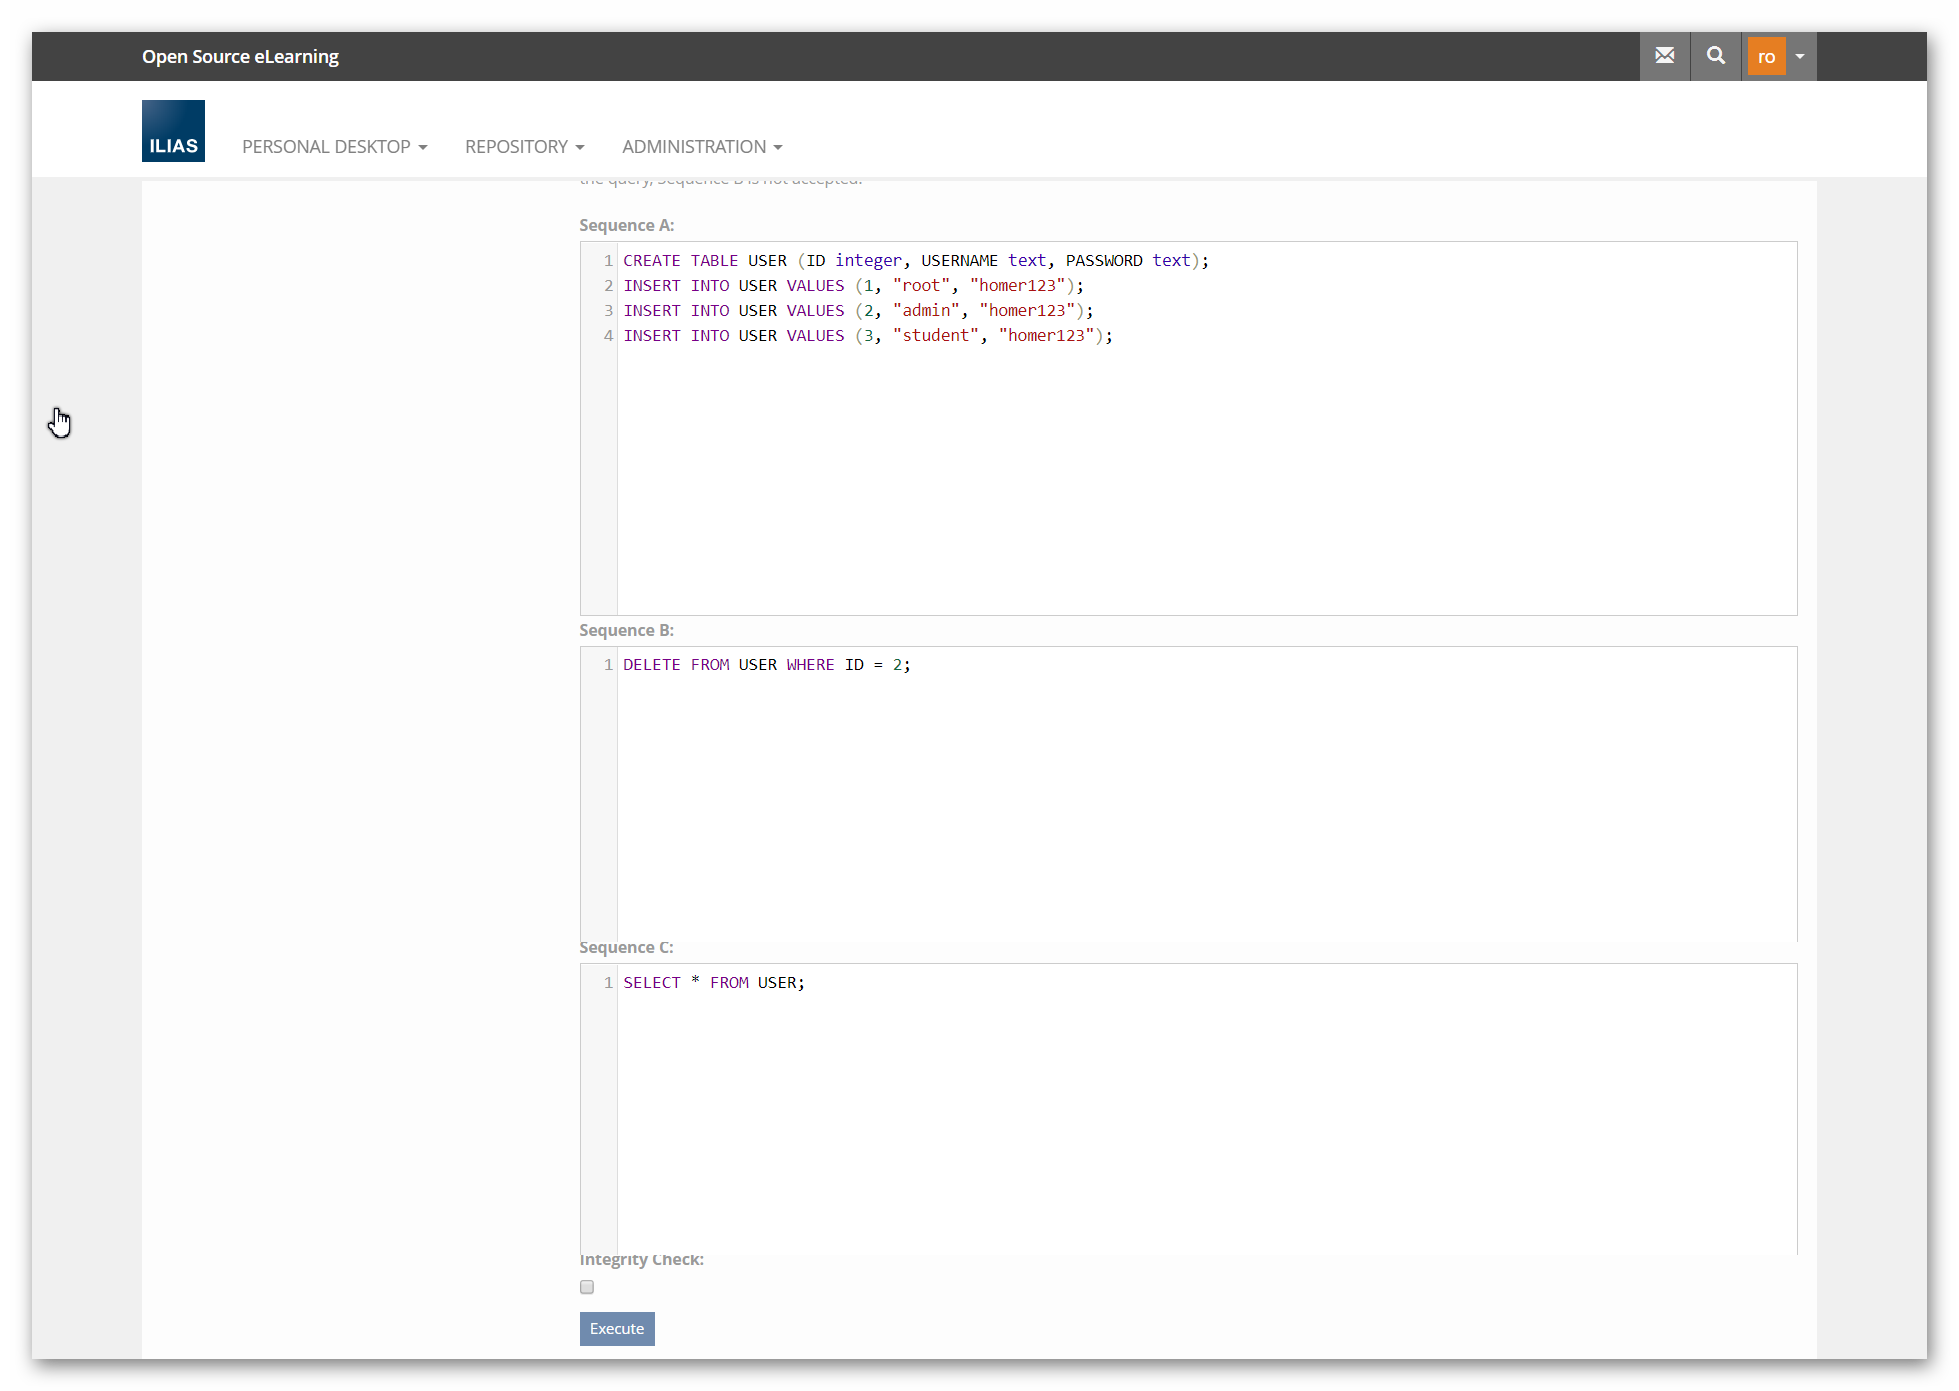
\includegraphics[page=1, width=0.7\paperwidth, trim=4 4 4 4, clip]{fig/Beispiel-SQL-Sequenzen-bei-DELETE-FROM-Anfrage.png} 
                \caption{SQL-Sequenzen im Falle einer DELETE FROM Anfrage (Beispiel)}
                \label{fig:beispiel-sql-sequenzen-bei-delete-from-anfrage}
            \end{center}
        \end{figure}
        
\subsection{Teil 2: Die Ausgabe}
            
        Die Ausgabe wird bei einem Druck auf \glqq\textit{Ausführen}\grqq\ (Englische Spracheeinstellung: \glqq\textit{Execute}\grqq ) automatisch erzeugt. Bei der Erstellung einer Frage ist zu beachten, dass in der Ausgabe keine Fehlermeldung anzeigen werden darf. Außerdem ist es selbstverständlich hilfreich die Ausgabe auf ein erwartetes Ergebnis zu überprüfen.
        
        \begin{figure}[H]
            \begin{center}
                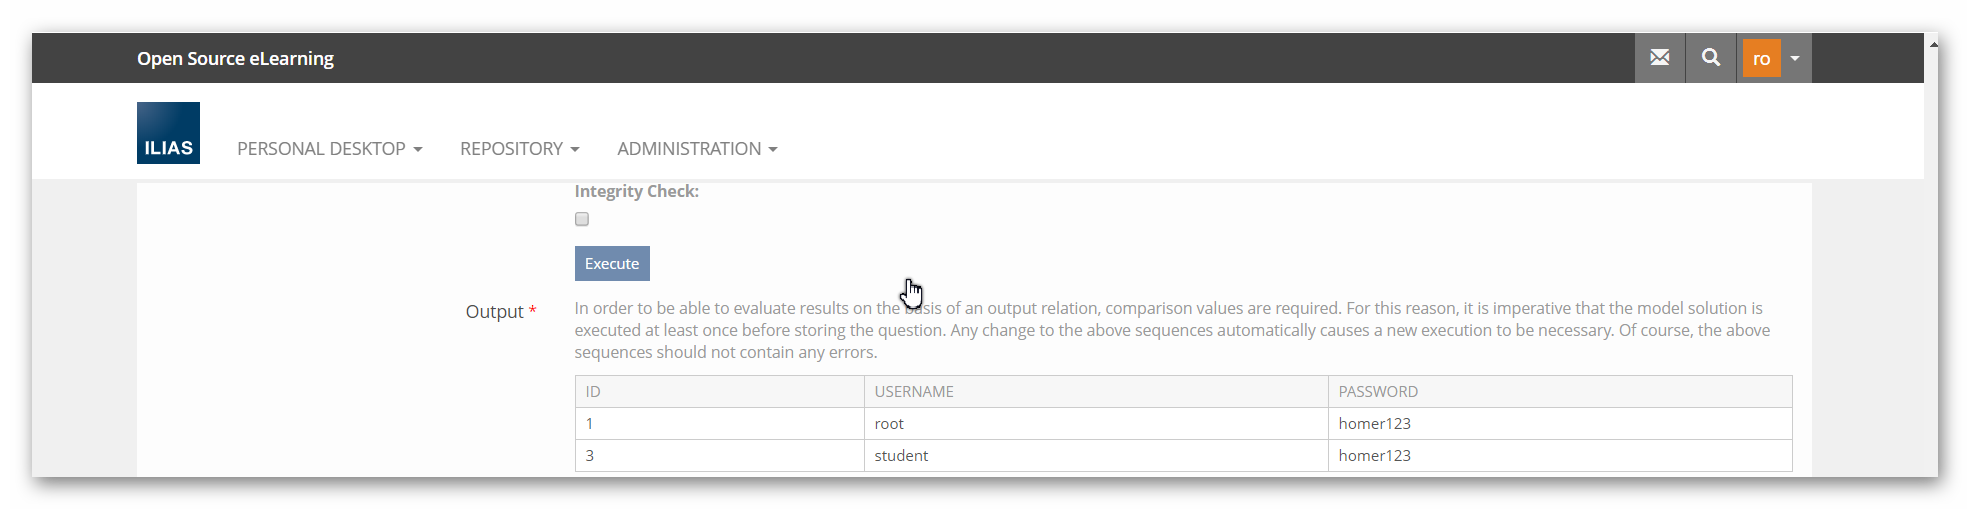
\includegraphics[page=1, width=0.7\paperwidth, trim=4 4 4 4, clip]{fig/Beispiel-Ausgabe-DELETE-FROM.png} 
                \caption{Ausgabe bei SQL-Sequenzen aus \textbf{Abbildung \ref{fig:beispiel-sql-sequenzen-bei-delete-from-anfrage}}}
                \label{fig:beispiel-ausgabe-delete-from-anfrage}
            \end{center}
        \end{figure}
        
\subsection{Teil 3: Die Bepunktung}

        Ein letzter wichtiger Teil, der bei der Erstellung einer Frage zu beachten ist, ist die Bepunktung. Allgemein gesprochen handelt es sich dabei um verschiedene Metriken, die jeweils über die letzte Ausgabe der Musterlösung und die letzte Ausgabe der Antwort des Teilnehmers gelegt werden, um eine Punktzahl für die jeweilige Antwort zu errechnen. Dabei kann der Frageersteller jeder verfügbaren Metrik eine gewisse Punktzahl zuteilen, die ein Teilnehmer maximal in Hinsicht auf diese Metrik erzielen kann. Die Punktzahlen der verschiedenen Metriken addieren sich dann zur Gesamtpunktzahl. Dabei muss die maximal mögliche Gesamtpunktzahl immer positiv sein, um eine Frage erfolgreich anzulegen. Das heißt, dass mindestens für eine verfügbare Metrik eine Maximalpunktzahl größer Null haben muss. 
        
        Zum Release von \eigenname{assSQLQuestion} sind insgesamt drei Metriken verfügbar: \glqq\textit{Anzahl der Tupel}\grqq\ (engl. \glqq\textit{Number of Tuples}\grqq), \glqq\textit{Namen der Attribute}\grqq\ (engl. \glqq\textit{Names of the attributes}\grqq) und \glqq\textit{Funktionale Abhängigkeiten}\grqq\ (engl. \glqq\textit{Functional Dependencies}\grqq). Die Funktionsweise dieser drei Metriken wird im Folgenden erläutert:
        
        \subsubsection{Anzahl der Tupel}
        
            Dies ist die technisch einfachste der drei Metriken. Hierbei werden die Tupel in der Ausgabe gezählt und miteinander verglichen. Hat die Ausgabe des Testteilnehmers identisch viele Tupel wie die Ausgabe der Musterlösung, so bekommt der Teilnehmer die maximale Punktzahl für diese Metrik, in jedem anderen Fall erhält er keine Punkte.
            
            \begin{figure}[H]
                \begin{center} 
                    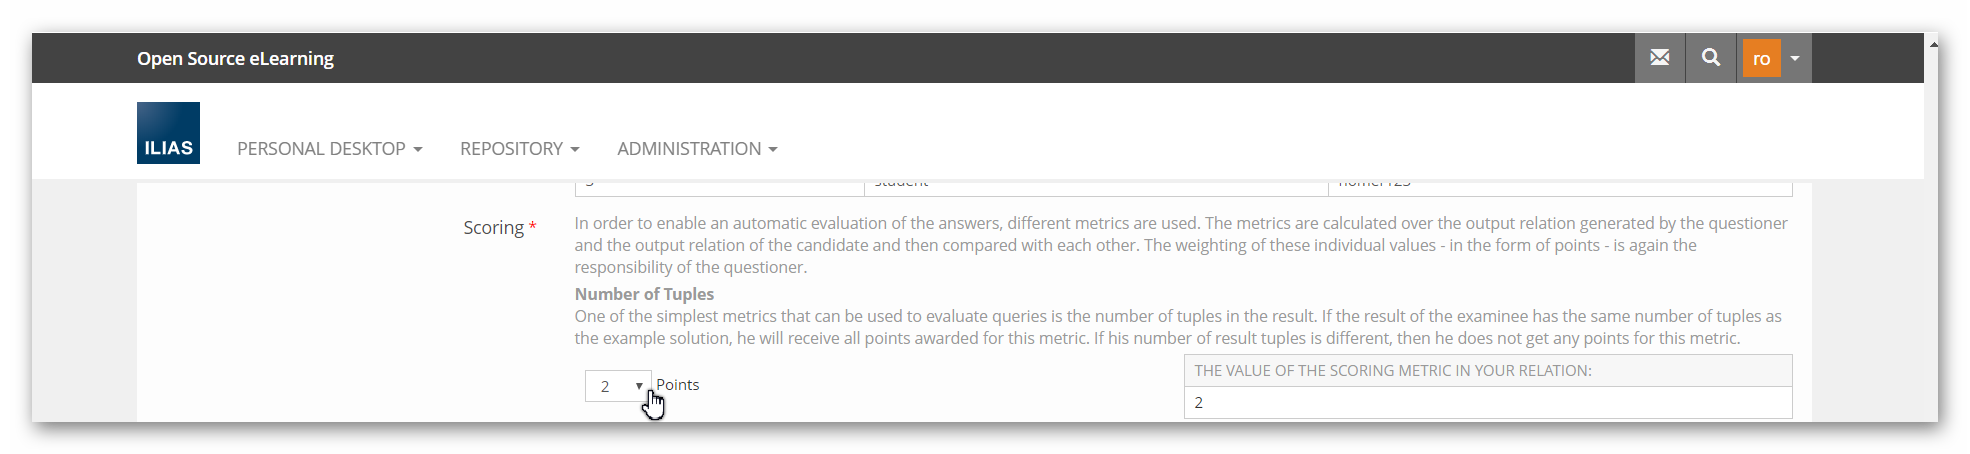
\includegraphics[page=1, width=0.7\paperwidth, trim=4 4 4 4, clip]{fig/Beispiel-Anzahl-der-Tupel-DELETE-FROM.png} 
                    \caption{Anzahl der Tupel zu \textbf{Abbildung \ref{fig:beispiel-sql-sequenzen-bei-delete-from-anfrage}}}
                    \label{fig:beispiel-anzahl-der-tupel-delete-from-anfrage}
                \end{center}
            \end{figure}
            
        \subsubsection{Namen der Attribute}
        
            Diese Metrik vergleicht die Bezeichner der Attribute miteinander. Dabei ist die Ordnung und auch die Groß-/Kleinschreibweise der Bezeichner irrelevant. Berechnet wird die Punktzahl über die Jaccard-Distanz: $ Punkte = MaxPunkte * (1 - JaccardDistanz) $. Es wird dabei nicht gerundet, wodurch auch im Gesamtergebnis mit ungerundeten Punktzahlen zu rechnen ist.
            
            Wenn Prüfungsteilnehmer ihre Bezeichner frei wählen dürfen, sollte die maximale Punktzahl bei dieser Metrik logischerweise Null entsprechen.
            
            \begin{figure}[H]
                \begin{center}
                    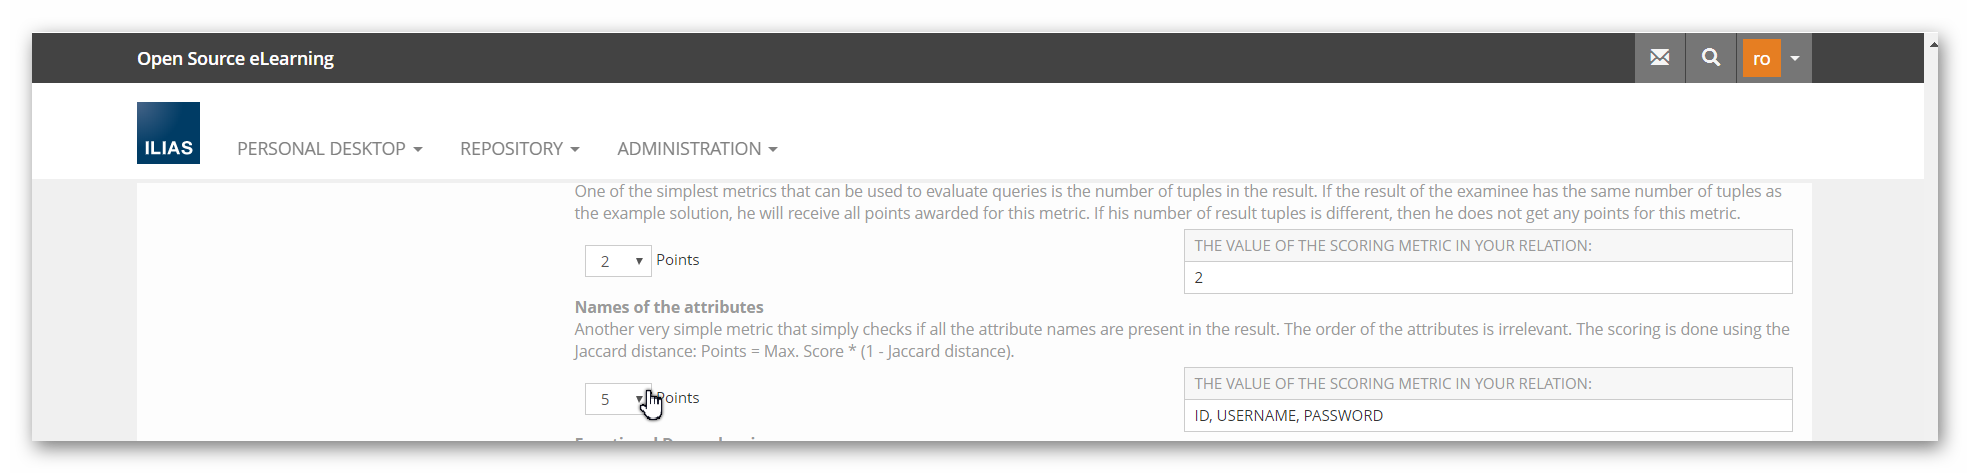
\includegraphics[page=1, width=0.7\paperwidth, trim=4 4 4 4, clip]{fig/Beispiel-Namen-der-Attribute-DELETE-FROM.png} 
                    \caption{Namen der Attribute zu \textbf{Abbildung \ref{fig:beispiel-sql-sequenzen-bei-delete-from-anfrage}}}
                    \label{fig:beispiel-namen-der-attribute-delete-from-anfrage}
                \end{center}
            \end{figure}
            
        \subsubsection{Funktionale Abhängigkeiten}
        
            Die Metrik zu den funktionalen Abhängigkeiten ist die komplexeste der drei Metriken. Dabei werden zu den Ausgaben zunächst alle enthaltenen funktionalen Abhängigkeiten bestimmt, wobei in einem zweiten Schritt alle \glqq nicht minimalen\grqq\ Abhängigkeiten entfernt werden. Genauer heißt das, dass funktionale Abhängigkeiten bei denen bereits ein Bestandteil der Determinante die gleichen Attribute bestimmt, nicht für die Metrik verwendet werden. 
            
            Der übrige Pool von funktionalen Abhängigkeiten innerhalb der Ausgabe der Musterlösung, wird dann der Menge aus funktionalen Abhängigkeiten aus dem Ergebnis des Teilnehmers gegenüber gestellt. Hier wird, wie bei der Metrik zu den Namen der Attribute, eine ordnungsignorierende Jaccard-Distanz verwendet. Auch die Groß-/Kleinschreibung wird ignoriert und die Reihenfolge der Attribute in den funktionalen Abhängigkeiten werden Reihenfolge insensitiv behandelt. Die berechnende Formel ist auch hier wieder: $ Punkte = MaxPunkte * (1 - JaccardDistanz) $.
            
            \begin{figure}[H]
                \begin{center}
                    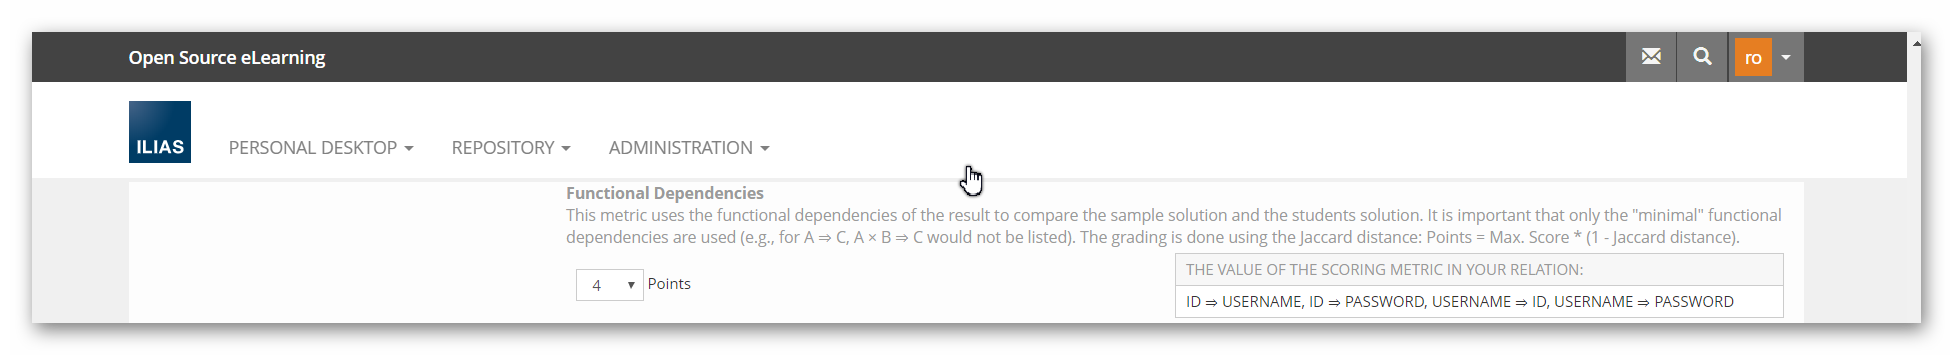
\includegraphics[page=1, width=0.7\paperwidth, trim=4 4 4 4, clip]{fig/Beispiel-Funktionale-Abhaengigkeiten-DELETE-FROM.png} 
                    \caption{Funktionale Abhängigkeiten zu \textbf{Abbildung \ref{fig:beispiel-sql-sequenzen-bei-delete-from-anfrage}}}
                    \label{fig:beispiel-funktionale-abhaengigkeiten-delete-from-anfrage}
                \end{center}
            \end{figure}